\let\RaggedRight\raggedright
\let\raggedright\relax
\documentclass[utf8,9pt,mathserif,usepdftitle=false]{beamer}
\usepackage[russian]{babel}

\newcommand{\dd}{\mathrm{d}}
\renewcommand{\Re}{\operatorname{Re}}
\renewcommand{\Im}{\operatorname{Im}}
\renewcommand{\exp}{\operatorname{e}}
\renewcommand{\imath}{\mathrm{i}}
\newcommand\Vect[1]{{\boldsymbol{#1}}}

% \input{present.daf}

% \setbeameroption{show notes on second screen}
\setbeameroption{hide notes}
\mode<presentation>
{
  \usetheme{default}
  %\usecolortheme{default} % dove, beaver
  \usecolortheme{whale}
  %\usefonttheme{serif}
}

\hypersetup{%
  pdfinfo={%
    Title={Lyapunov conference, IDSTU},%
    Subject={Spin degrees of freedom for fermion systems},%
    Author={Даниил Кучеров},%
    Keywords={fermion polarization;fermion spinor projection}%
  }
}

\title{Зависимость вероятности выживания электронного нейтрино от углов
  смешивания}%
\author{\underline{Кучеров Д.А.}\\[7em]\raggedleft\footnotesize Научный руководитель:
  Ломов В.П.\\%
}%
\date[ИГУ, 2025]{\vfill%\\[4ex]%
  \small{}Иркутск, 2025}

\begin{document}
\begin{frame}
  \titlepage
\end{frame}

\begin{frame}
	\frametitle{Задачи работы}
  В работе поставленно несколько задач:
  \begin{itemize}
  \item<2-> Ознакомится с теорией нейтринных осцилляций в среде.
  \item<3-> Провести вычисления с помощью метода разложения Магнуса, варьируя
    значения углов смешивания.
  \item<4-> Проанализировать полученные данные.
  \end{itemize}
\end{frame}

\begin{frame}
	\frametitle{Теоретическая часть}%
  Нейтрино — это нейтральные частицы имеющие полуцелый спин относящиеся к классу
  лептонов. Феноменологически выделяют два типа нейтрино: участвующие в
  взаимодействии — флейворные и участвующие в распространении в пространстве —
  массивные.

  \onslide<2->%
	Нейтрино существуют в трёх флейворах: электронные, мюонные и
  тау-нейтрино. Каждый флейвор ассоциируется с соответствующим лептоном
  (электроном, мюоном и тау-лептоном).

  \onslide<3->%
  Флейворные нейтрино можно считать линейной комбинацией массивных, справедливо и 
  обратное. Данная линейная комбинация может быть выражена с помощью унитарной
  матрицы смешивания \(U\)
  \begin{equation}
  	|\nu_{\alpha}\rangle=\sum_{i}U_{\alpha i}^{*}|\nu_{i}\rangle.
  \end{equation}

\end{frame}

\begin{frame}
	\frametitle{Нейтринные осцилляции}%
	Самая необычная черта нейтрино — это их осцилляции.

  \onslide<2->%
  Осцилляции нейтрино — периодические переходы между флейворами этих частиц,
  распространяющихся в веществе или в вакууме.

  \onslide<3->%
  Нейтринные осцилляции возможны, поскольку нейтрино массивны.%, и при этом
  % имеется смешивание между поколениями, аналогичное смешиванию между кварками.
\end{frame}

\begin{frame}
  \frametitle{Осцилляции в вакууме}%
  Массивные нейтрино подчиняются уравнению
	\begin{equation}
		H|\nu_{i}(t)\rangle=\imath\frac{\dd}{\dd t}|\nu_{i}(t)\rangle=
		E_{i}|\nu_{i}(t)\rangle, \qquad E_{i}=\sqrt{\Vect{p}^{2}+m_{i}^{2}}.
	\end{equation}

  \onslide<2->%
	Решением является следующее выражение
	\begin{equation}
		|\nu_{i}(t)\rangle=\exp^{-\imath E_{i}t}|\nu_{i}(0)\rangle.
	\end{equation}

  \onslide<3->%
	Положив, что в начальный момент времени нейтрино имело флейвор
  \(\alpha\), получим, что в момент времени \(t\) это состояние имеет вид
	\begin{equation}
		|\nu_{\alpha}(t)\rangle=\sum_{i}U_{\alpha i}^{*}\exp^{-\imath E_{i}t}|\nu_{i}\rangle.
	\end{equation}
\end{frame}

\begin{frame}
	\frametitle{Осцилляции в веществе}%
	Когда нейтрино распространяются в веществе, на их эволюционное уравнение
  влияют эффективные потенциалы взаимодействия со средой посредством реакций
  нейтрального и заряженного токов
    \begin{align*}
  	\nu_{l}(\overline{\nu}_{l})+N\xrightarrow[\text{CC}]{}l^{-}(l^{+})+\text{адроны}\\[2ex]
  	\nu_{l}(\overline{\nu}_{l})+N\xrightarrow[\text{NC}]{}\nu_{l}(\overline{\nu}_{l})+\text{адроны}.
  \end{align*}
  \onslide<2->%
	Влияние среды можно описать в терминах потенциалов, в которых
	распространяются нейтрино. Учитывая данные обстоятельства, было выведено
	уравнение для амплитуд массовых состояний:
	\onslide<3->%
	\begin{equation}\label{eq:2}
		\imath\frac{\dd\psi}{\dd\xi}=[H_{0}+\nu(\xi)W]\psi, 
		\qquad
		 W=
		\begin{pmatrix}
			c_{13}^{2}c_{12}^{2} & c_{12}s_{12}c_{13}^{2} & c_{12}c_{13}s_{13}\\
			c_{12}s_{12}c_{13}^{2} & s_{12}^{2}c_{13}^{2} & s_{12}c_{13}s_{13}\\
			c_{12}s_{13}c_{13} & s_{12}c_{13}s_{13} & s_{13}^{2}
		\end{pmatrix}.
	\end{equation}
\end{frame}

\begin{frame}
	\frametitle{Особенности уравнения нейтринных осцилляций}%
  \begin{enumerate}
  \item<1-> Уравнение матричное.
  \item<2-> \(H(\xi)=[H_{0}+\nu(\xi)W]\) — это унитарная матрица гамильтониана
    эволюции.
  \item<3-> Технически ответ может может быть записан в виде некоторой матричной
    экспоненты
    
    \begin{equation}
    	\Psi(r)=\exp^{\frac{-\imath LH}{\hbar}}\Psi(r_{*})
    \end{equation}
  \end{enumerate}
\end{frame}

\begin{frame}
	\frametitle{Генерирование и обработка данных}%
	Нас интересует
	\begin{itemize}
		\item<2-> Характер зависимости вероятности выживания электронного нейтрино от 
		углов смешивания
	\end{itemize}
	\onslide<3->%
	Для этого мы
	\begin{itemize}
		\item<4-> Интегрируем уравнение нейтринных осцилляций варьируя отдельно значения 
		каждого угла, используя алгоритм М4 и сценарий bash-оболочки.
		\item<5-> Обрабатываем полученные данные, используя сценарий bash-оболочки.
	\end{itemize}
	\onslide<6->%
	Современные значения углов смешивания
	\begin{align*}
		\sin^{2}{\theta_{12}}=0,307_{-0,012}^{+0,013}\\
		\sin^{2}{\theta_{23}}=0,417_{-0,028}^{+0,025}\\
		\sin^{2}{\theta_{13}}=0,0212\pm 0,0008
	\end{align*}
  \onslide<7->%
  В сценариях для генерации и обработки данных в основу легли следующие формулы
  \begin{align*}
  		\sin{\theta_{f}}=f\cdot\sin{\theta}\\
  		\eta_{f}=\frac{\Prob_{f}-\Prob_{0}}{\Prob_{0}}
  \end{align*}
  
\end{frame}

\begin{frame}
	\begin{figure}[h]
		\centering
		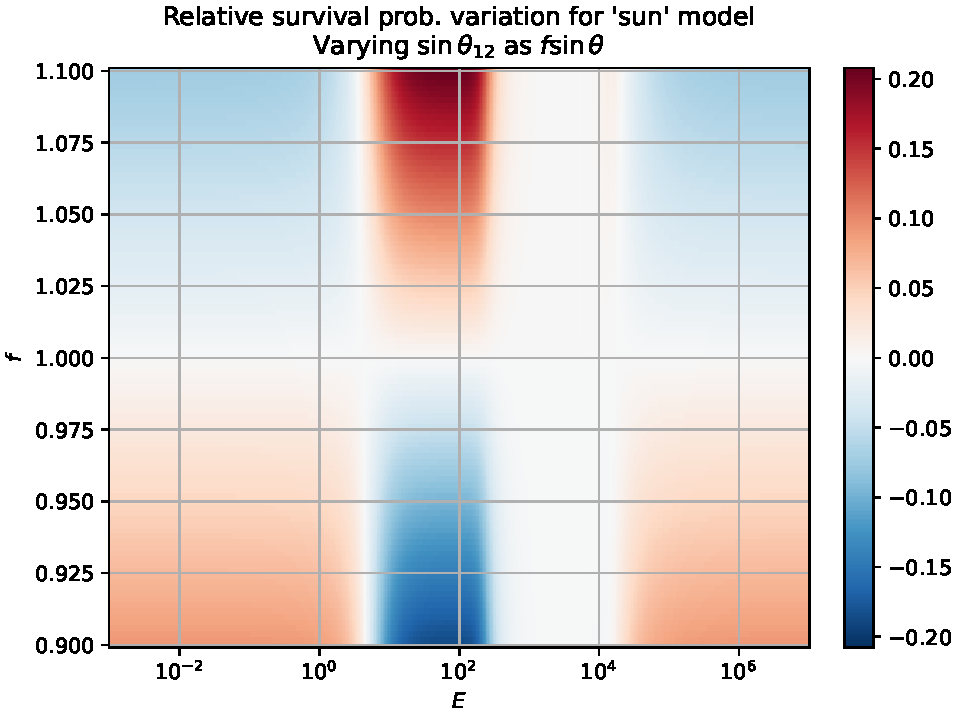
\includegraphics[width=0.8\linewidth]{sun-in-ang12}
		\caption{График относительного отклонения \(\langle P_{ee}\rangle\) при
      вариации угла \(\theta_{12}\) }
	\end{figure}
\end{frame}

\begin{frame}
	\begin{figure}[h]
		\centering
		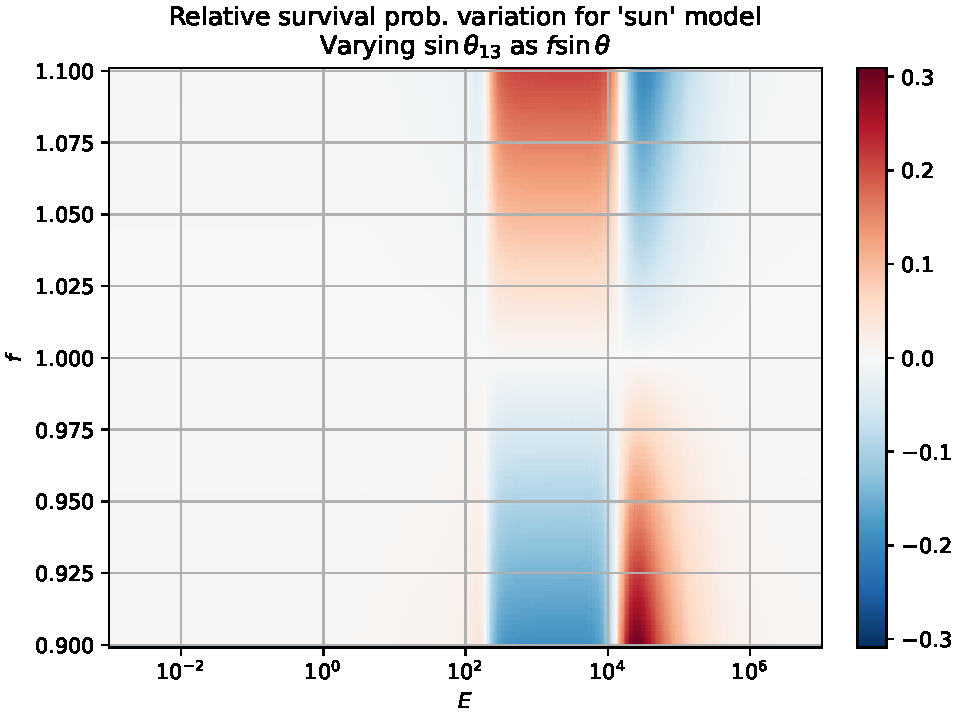
\includegraphics[width=0.8\linewidth]{sun-in-ang13}
		\caption{График относительного отклонения \(\langle P_{ee}\rangle\) при
      вариации угла \(\theta_{13}\)}
	\end{figure}
\end{frame}

\begin{frame}
	\frametitle{Выводы}
	\begin{itemize}
  \item<1-> Разобран механизм осцилляций нейтрино в вакууме и в веществе.
  \item<2-> Разработаны сценарии для автоматизации расчётов и сценарии для
    визуализации полученных данных .
   \item<3-> Выделены области наибольшей чувствительности вероятности выживания от 
   углов смешивания \(\theta_{12}\) и \(\theta_{13}\).
	\end{itemize}
\end{frame}

\begin{frame}
	\frametitle{Перспективы работы}
	\begin{itemize}
  \item<1-> Провести анализ для других типов нейтрино.
  \item<2-> Провести анализ с вариацией параметров профиля плотности.
  \item<3-> Рассмотреть случай прохождения нейтрино сквозь вещество. 
  \item<4-> Разработать формулы для анализа корреляций в вариациях.
	\end{itemize}
\end{frame}

\begin{frame}
  \frametitle{КОНЕЦ}%
  \LARGE\centering\bfseries
  СПАСИБО ЗА ВНИМАНИЕ!
\end{frame}

\begin{frame}
  \frametitle{Дополнительный материал}%
  Реакции с нейтрино в веществе
  \begin{align*}
    \nu_{l}(\overline{\nu}_{l})+N\xrightarrow[\text{CC}]{}l^{-}(l^{+})+\text{адроны}\\[2ex]
    \nu_{l}(\overline{\nu}_{l})+N\xrightarrow[\text{NC}]{}\nu_{l}(\overline{\nu}_{l})+\text{адроны}.
  \end{align*}
  	Вероятность перехода флейвора нейтрино от \(\alpha\) к \(\beta\) запишется
  \begin{equation}
  	P_{\alpha \beta}=|\psi_{\beta}(r)|^{2}
  \end{equation}
  \onslide<2->%
  Амплитуда вероятности обнаружения состояния флейвора частицы \(\nu_{j}\) запишется
  \begin{equation}
  	\psi_{\beta}(r)=\sum_{j=1}^{3}U_{\beta j}A_{j}\exp^{-\imath E_{j}L}, \qquad L=r-r_{*}
  \end{equation}
    \onslide<2->%
  Состояние системы \(|\psi(t)\rangle\) во время \(t \geqslant t_{0}\) может быть выражено как
  \begin{equation}
  	|\psi(t)\rangle=\sum_{\beta}\psi_{\beta}(t)|\nu_{\beta}\rangle
  \end{equation}
  с условием \(\psi_{\beta}(t_{0})=\delta_{\alpha \beta}\).
\end{frame}

\end{document}

%%% Local Variables:
%%% mode: latex
%%% fill-column: 80
%%% TeX-master: t
%%% TeX-PDF-mode: t
%%% End:
%%% vim: syn=tex ft=tex tw=80 ts=2 sw=2 et:
